% !TeX program = xelatex
% ============================================================================
%  全国大学生数学建模竞赛（CUMCM）论文 LaTeX 模板
% ----------------------------------------------------------------------------
%  编译方式（必须用 XeLaTeX，中文需要它）：
%    本地 TeX Live：  latexmk -xelatex main.tex
%    或直接两次：     xelatex main.tex  →  xelatex main.tex   （第二次生成目录/引用）
%    Overleaf：       菜单 -> 编译器 选择 "XeLaTeX"，然后重新编译
%
%  使用步骤：
%    1. 把本次赛题内容填入正文各章节（标注了 % ===== 的地方）。
%    2. 图片统一放进 Pictures/ 对应题目的文件夹，正文用
%       \includegraphics[width=...]{Pictures/Question1/你的图.png} 引用。
%    3. 参考文献写入 references.bib，正文用 \cite{键名} 引用。
%    4. 附录里贴入本题的求解代码与支撑材料清单。
%
%  字体：SIMLI.TTF、lishugbk.ttf 已与本文件放在同一目录（可选，未使用不影响编译）。
% ============================================================================

\documentclass[a4paper,12pt]{article}

% ---------------- 中文支持 ----------------
\usepackage{ctex}                      % 中文排版，提供 \songti \heiti \zihao 等
\usepackage{fontspec}
\usepackage{xeCJK}
% 修复：ctex 的 Windows 字体集未给 \songti（宋体族）配置加粗字形，
% 导致 \textbf{中文} 不生效。这里为宋体补上"加粗=黑体"映射；
% 若当前系统没有 SimSun（如 Overleaf 的 fandol 字体），则跳过（fandol 自带加粗）。
\IfFontExistsTF{SimSun}{%
  \setCJKfamilyfont{zhsong}{SimSun}[BoldFont=SimHei]%
}{}
% 可选中文艺术字体（本模板未使用，保留以备需要）：
\newCJKfontfamily\lsfont[Path=./, UprightFont=*]{lishugbk.ttf}   % 隶书
\newfontfamily\simliFont[Path=./]{SIMLI.TTF}                      % SimLi 隶变

% ---------------- 页面设置（国赛 A4 页边距） ----------------
\usepackage[top=2.54cm, bottom=2.54cm, left=3cm, right=3cm]{geometry}

% ---------------- 数学公式 ----------------
\usepackage{amsmath, amssymb, bm}
\usepackage{siunitx}                  % 单位排版

% ---------------- 表格 ----------------
\usepackage{array}
\usepackage{booktabs}                 % 三线表
\usepackage{tabularx}
\usepackage{multirow}
\usepackage{makecell}
\usepackage{threeparttable}
\usepackage[table]{xcolor}            % 表格颜色（含 colortbl）
\definecolor{accent}{RGB}{31,78,121}  % 强调色（可选）

% ---------------- 图片与浮动 ----------------
\usepackage{graphicx}
\usepackage{float}
\floatplacement{figure}{H}            % 图默认固定位置（去掉可自动浮动）
\floatplacement{table}{H}             % 表默认固定位置
\usepackage{caption}
\usepackage{subcaption}               % 并排子图
\usepackage[section]{placeins}

% ---------------- 目录与章节格式 ----------------
\usepackage[titles]{tocloft}
\usepackage{titlesec}
\usepackage{setspace}

% 目录标题：黑体三号居中
\renewcommand{\cfttoctitlefont}{\hfill\heiti\zihao{3}}
\renewcommand{\cftaftertoctitle}{\hfill}
% 目录条目：宋体小四
\renewcommand{\cftsecfont}{\songti\zihao{-4}}
\renewcommand{\cftsubsecfont}{\songti\zihao{-4}}
\renewcommand{\cftsecpagefont}{\songti\zihao{-4}}

% 编号格式：一级用中文（一、二、三），二级用 1.1、1.2
\renewcommand{\thesection}{\chinese{section}}
\renewcommand{\thesubsection}{\arabic{section}.\arabic{subsection}}
\renewcommand{\thesubsubsection}{\arabic{section}.\arabic{subsection}.\arabic{subsubsection}}

% 一级标题：黑体四号居中
\titleformat{\section}
  {\heiti\zihao{4}\centering}
  {\chinese{section}、}
  {0em}
  {}
% 二级标题：宋体小四顶格加粗
\titleformat{\subsection}
  {\songti\zihao{-4}\bfseries}
  {\arabic{section}.\arabic{subsection} }
  {0em}
  {}
% 三级标题：黑体小四缩进2字符（黑体本身即粗，无需再加 \bfseries）
\titleformat{\subsubsection}
  {\heiti\zihao{-4}}
  {\hspace{2em}\arabic{section}.\arabic{subsection}.\arabic{subsubsection} }
  {0em}
  {}
\setcounter{secnumdepth}{3}

% ---------------- 参考文献 ----------------
\usepackage[super, square]{natbib}    % 上标数字引用
\bibliographystyle{unsrtnat}

% ---------------- 超链接 ----------------
\usepackage{hyperref}
\hypersetup{
    colorlinks=true,
    linkcolor=black,
    filecolor=magenta,
    urlcolor=cyan,
    citecolor=blue,
    pdftitle={数学建模论文},
}

% ---------------- 代码排版 ----------------
\usepackage{listings}
\lstset{
    basicstyle=\ttfamily\small,
    breaklines=true,
    frame=single,
    numbers=left,
    commentstyle=\color{green},
    keywordstyle=\color{blue},
    stringstyle=\color{red},
}

% ---------------- 其他常用宏包 ----------------
\usepackage{enumitem}                 % 自定义列表
\usepackage{multicol}                 % 多栏
\usepackage{ragged2e}
\usepackage{prettyref}
\usepackage[many]{tcolorbox}          % 彩色步骤框
\tcbuselibrary{listings, breakable}
\usepackage[absolute,overlay]{textpos}

% 可选：强调宏
\newcommand{\attr}[1]{\textcolor{accent}{\textbf{#1}}}

% ============================================================================
\begin{document}

% 正文字号：宋体小四
\songti\zihao{-4}
\setlength{\parindent}{2em}

% ==================== 一、题目（替换为本次赛题标题） ====================
\begin{center}
    \setstretch{1.5}
    \songti\zihao{4}
    \heiti\zihao{3} 基于XXX模型的XXXXXX问题研究
\end{center}

% ==================== 二、摘要 ====================
\begin{center}
  \heiti\zihao{4} 摘\quad 要
\end{center}

{
\songti\zihao{-4}      % 摘要正文：宋体小四
\setlength{\parindent}{2em}

% ---- 第一段：总体概括（研究对象、总体思路、主要模型、核心结论） ----
本文针对\underline{XXXXXX}问题进行研究。基于\underline{XXXXXX}原理，
结合题目提供的数据，分别建立了\underline{XXX模型}与\underline{XXX模型}，
设计了相应的求解算法，并对\underline{XXX}进行了计算与可靠性分析。

% ---- 之后按"对于问题一 / 问题二 / 问题三"分段，写出每题的方法与关键结果 ----
\textbf{对于问题一}，\underline{简要说明问题一的建模思路、所用方法与求解结果}。

\textbf{对于问题二}，\underline{简要说明问题二的建模思路、所用方法与求解结果}。

\textbf{对于问题三}，\underline{简要说明问题三的建模思路、所用方法与求解结果}。

最后，对模型的优缺点进行评价，并提出改进的方向。

\textbf{关键词：}关键词一\quad 关键词二\quad 关键词三\quad 关键词四
}

\clearpage

% ==================== 目录（国赛正文通常不含目录，如需可取消注释） ====================
% \tableofcontents
% \clearpage

% ==================== 一、问题的提出和重述 ====================
\section{问题的提出和重述}

\subsection{问题的提出}
\underline{介绍问题背景：}该项问题的实际工程/科学背景，为什么重要，现有方法存在什么困难，
因此需要建立科学、可靠的模型。

\subsection{问题的重述}
\underline{用自己的话重新陈述赛题，并把赛题给出的若干个子问题逐条列出。}

\textbf{问题1：}\underline{重述问题1的要求。}

\textbf{问题2：}\underline{重述问题2的要求。}

\textbf{问题3：}\underline{重述问题3的要求。}

% ==================== 二、问题的分析 ====================
\section{问题的分析}

\underline{整体分析思路，可配合一张流程图（见下方示例）。}

\textbf{针对问题一：}\underline{分析问题一的难点与解题思路。}

\textbf{针对问题二：}\underline{分析问题二的难点与解题思路。}

\textbf{针对问题三：}\underline{分析问题三的难点与解题思路。}

\textbf{建模思路与框架：}本文的整体建模流程如下图所示。

\begin{figure}[H]
\centering
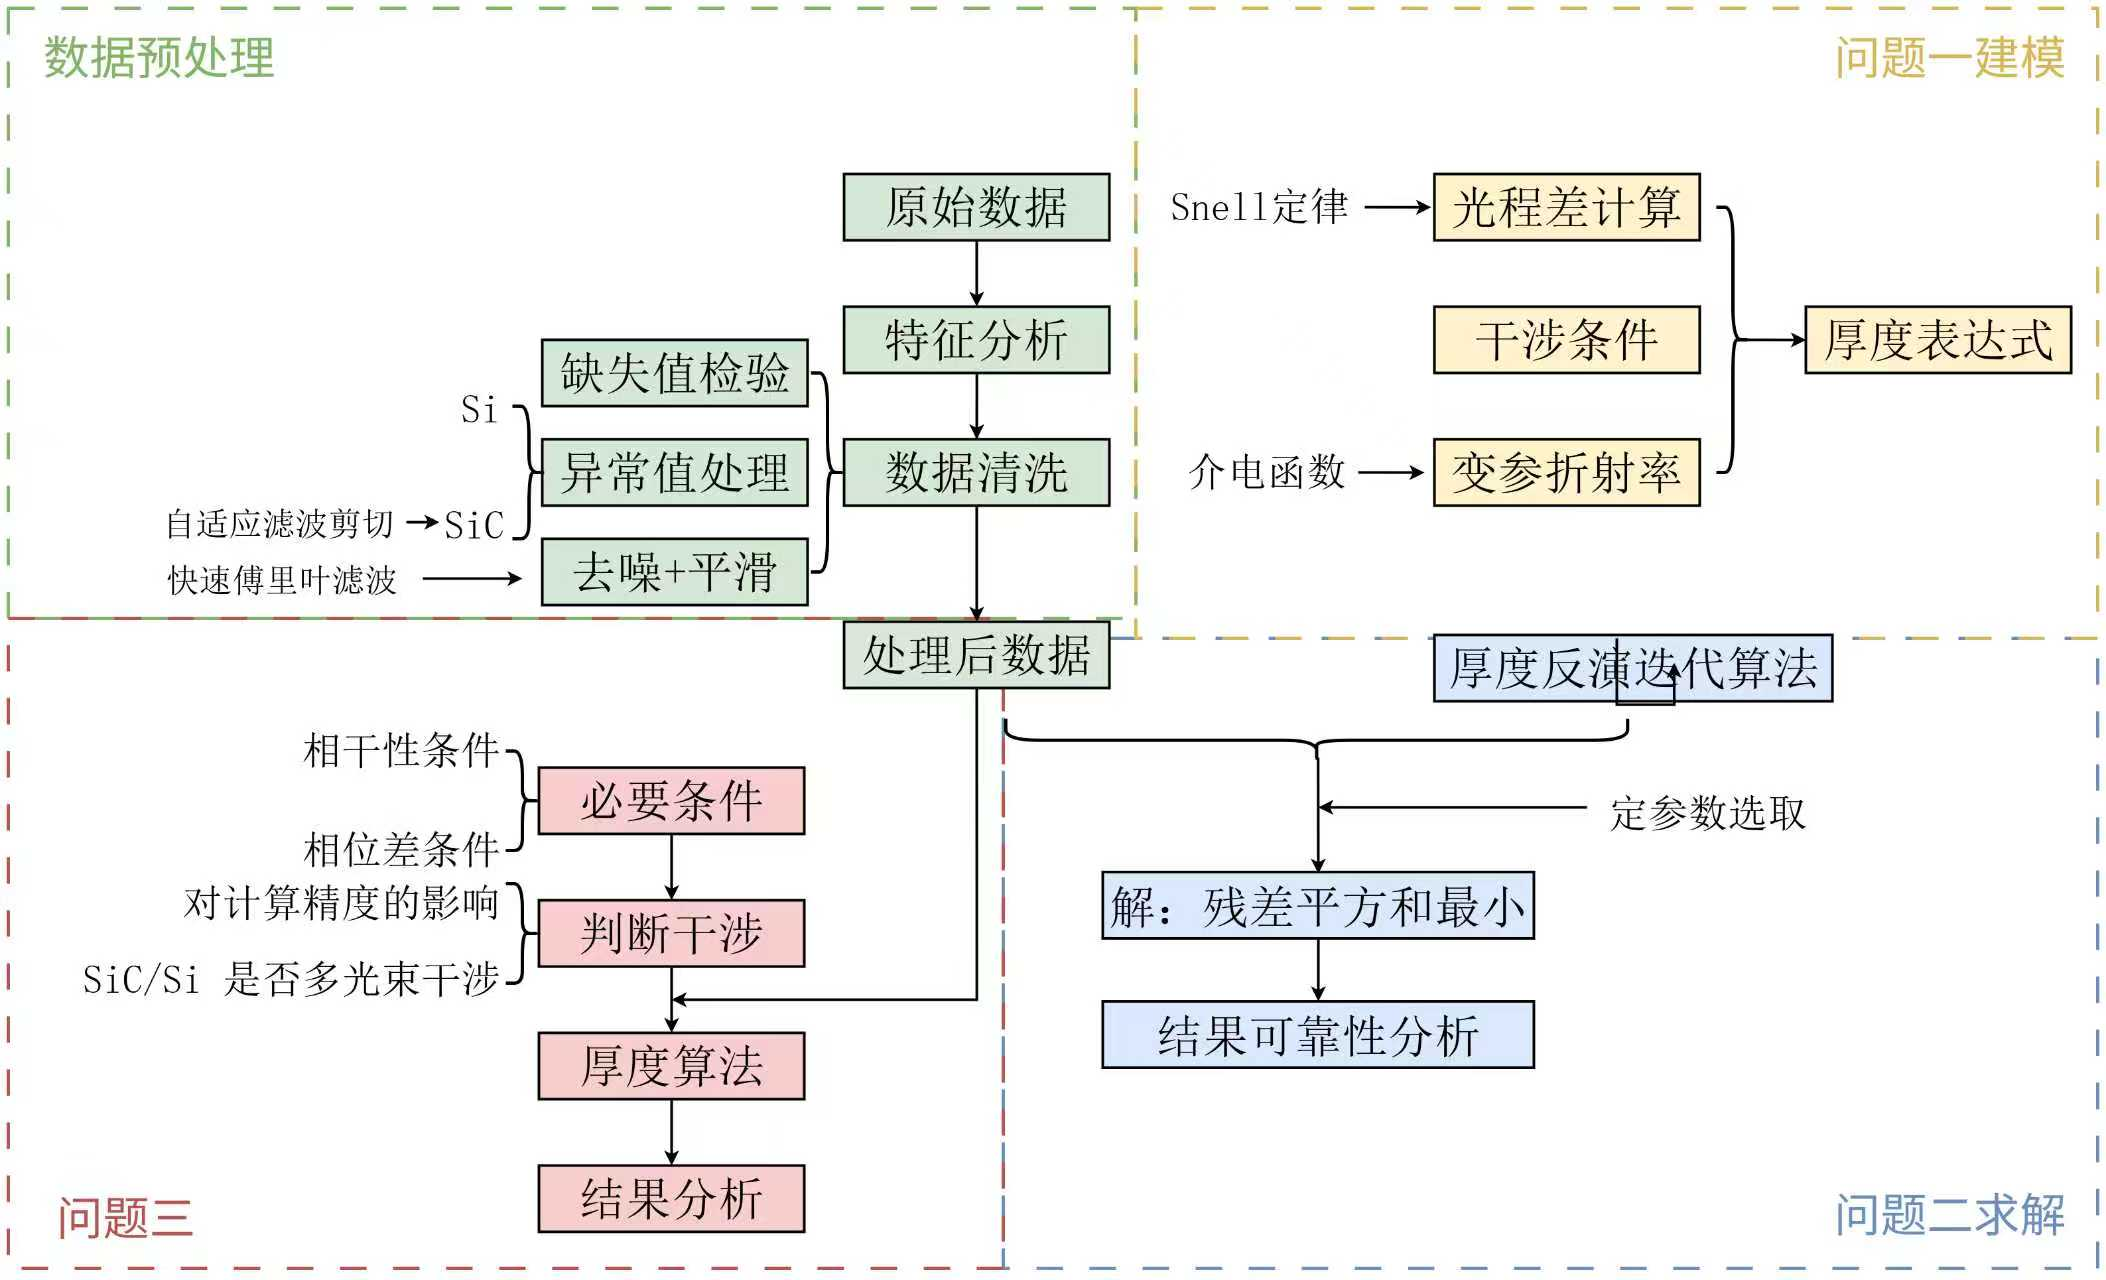
\includegraphics[width=0.9\textwidth]{Pictures/流程图示例.jpg}
\caption{整体建模流程图（此处为示例图，请替换为你自己的流程图）}
\label{fig:flow}
\end{figure}

% ==================== 三、模型假设 ====================
\section{模型假设}

\begin{enumerate}[label=\arabic*., itemsep=0pt, topsep=2pt]
    \item \underline{假设……（使问题简化且合理的假设，逐条列出，4~6条为宜）}。
    \item \underline{假设……}。
    \item \underline{假设……}。
    \item \underline{假设……}。
\end{enumerate}

% ==================== 四、符号说明 ====================
\section{符号说明}

\begin{table}[H]
    \centering
    \setlength{\heavyrulewidth}{1.5pt}  % 顶/底线1.5磅
    \setlength{\lightrulewidth}{1pt}    % 中间线1磅
    \captionsetup{skip=0pt}
    \begin{tabularx}{\textwidth}{>{\centering\arraybackslash}X>{\centering\arraybackslash}X>{\centering\arraybackslash}X}
        \toprule[1.5pt]
        \textbf{符号} & \textbf{说明} & \textbf{单位} \\
        \midrule[1pt]
        % ---- 按需添加本论文用到的所有符号 ----
        $d$        & 待求参数（示例） & 无量纲 \\
        $n$        & 折射率（示例）   & 无量纲 \\
        $\theta$   & 入射角（示例）   & $^\circ$ \\
        $\lambda$  & 波长（示例）     & $\mu$m \\
        \bottomrule[1.5pt]
    \end{tabularx}
\end{table}

% ==================== 五、数据的处理 ====================
\section{数据的处理}

\subsection{数据整体分析}
\underline{描述数据的规模、来源、特点，可先画出数据整体分布图，说明观察到的规律。}

\subsection{数据清洗与处理流程}

\subsubsection{缺失值检验}
\underline{说明数据是否存在缺失、如何处理。}

\subsubsection{异常值处理}
\underline{说明是否存在异常值、如何识别并剔除。}

\subsubsection{数据去噪}
\underline{如有需要，说明采用的去噪/平滑方法。}

\subsubsection{数据转换}
\underline{说明为建模所做的单位换算、无量纲化等数据转换。}

% ==================== 六、模型建立和求解 ====================
\section{模型建立和求解}

\subsection{问题一：\underline{问题一的标题}}

\subsubsection{问题一：模型建立}
\underline{推导公式（逐式编号、说明物理意义）、引用文献\cite{key_example}，配示意图。}

示例公式：
\begin{equation}
    y = a x + b
    \label{eq:example}
\end{equation}

其中，$a$、$b$ 为待定系数。按式（\ref{eq:example}）……

\subsubsection{问题一：模型求解}
\underline{说明求解算法与步骤（可用 tcolorbox 分步骤展示），给出结果。}

\begin{tcolorbox}[colframe=black]
\textbf{Step1: } \underline{第一步做什么}

\textbf{Step2: } \underline{第二步做什么}

\textbf{Step3: } \underline{第三步做什么}
\end{tcolorbox}

结果如表\ref{tab:example}所示：

\begin{table}[H]
    \centering
    \caption{问题一求解结果（示例）}
    \label{tab:example}
    \begin{tabularx}{\textwidth}{>{\centering\arraybackslash}X>{\centering\arraybackslash}X>{\centering\arraybackslash}X}
        \toprule
        参数 & 结果1 & 结果2 \\
        \midrule
        $d$ & 3.28 & 3.24 \\
        $R^2$ & 0.873 & 0.877 \\
        \bottomrule
    \end{tabularx}
\end{table}

\subsubsection{问题一：结果分析与可靠性验证}
\underline{一致性检验、残差分析、物理合理性等角度评价结果。}

\subsection{问题二：\underline{问题二的标题}}
\underline{按照"建模—求解—结果分析"的思路组织问题二。}

\subsection{问题三：\underline{问题三的标题}}
\underline{按照"建模—求解—结果分析"的思路组织问题三。}

% ==================== 七、模型的评价和改进 ====================
\section{模型的评价和改进}

\subsection{模型的评价}
\subsubsection{优点}
\underline{模型的物理意义明确、算法鲁棒性好、结果可靠等优点。}

\subsubsection{缺点}
\underline{模型依赖的参数、计算复杂度、适用范围等不足。}

\subsection{模型的改进}
\underline{提出改进方向，如引入更精细的模型、更优的求解算法等。}

% ==================== 八、模型的推广和应用 ====================
\section{模型的推广和应用}
\underline{说明模型在其他场景/领域的应用价值。}

% ==================== 参考文献 ====================
\addcontentsline{toc}{section}{参考文献}
\bibliography{references.bib}

\clearpage

% ==================== 附录 ====================
\section*{附录}

\subsection*{支撑材料列表}
\begin{multicols}{2}
\begin{enumerate}
    \item \underline{示意图、结果图等图片文件}
    \item \underline{各问的求解代码文件}
    \item \underline{数据表格文件}
\end{enumerate}
\end{multicols}

\clearpage

\subsection*{问题一求解代码}

% 代码块模板：把真实代码粘贴到 lstlisting 环境里（注意不能用表格式代码块过多，避免页数超限）
\begin{table}[H]
    \centering
    \setlength{\heavyrulewidth}{1.5pt}
    \setlength{\lightrulewidth}{1pt}
    \renewcommand{\arraystretch}{1.2}
    \begin{tabular}{>{\centering\arraybackslash}p{0.92\textwidth}}
        \toprule[1.5pt]
        \textbf{问题一求解代码（1）} \\
        \midrule[1pt]
        运行环境：MATLAB R2024b \\
        \midrule[1pt]
        \begin{lstlisting}[
            language=MATLAB,
            basicstyle=\ttfamily,
            frame=none,
            breaklines=true,
            breakatwhitespace=true,
        ]
% ===== 在此粘贴问题一的求解代码 =====
clear; close all; clc;
disp('Hello CUMCM');
        \end{lstlisting} \\
        \bottomrule[1.5pt]
    \end{tabular}
\end{table}

% ===== 附录如需更多代码块，复制上面的表格模板即可 =====

\end{document}
